\chapter{Descripción de Broadsea}

%ATLAS es una plataforma de análisis de datos de ciencia abierta perteneciente a la red OHDSI para facilitar el intercambio de estructuras de análisis entre organizaciones pertenecientes a esta misma red. ATLAS se sostiene sobre el modelo de datos común de OMOP (CDM) que es el objeto de unión de todos los estudios OHDSI, la normalización de las bases de datos a este estándar clínico.

%Para facilitar la implementación de ATLAS, OHDSI propone diversas alternativas dependiendo de las necesidades de la organización interesada. En este manual se presenta la implementación, instalación, despliegue y configuración a través de Broadsea.

Broadsea es un proyecto basado en Docker que permite desplegar un entorno de herramientas, configuraciones y dependencias OHDSI de la manera más sencilla hasta el momento. De hecho, la misma organización la presenta, textualmente, como \textit{''la forma más sencilla de instalar (y actualizar) las herramientas OHDSI"} \cite{Broadsea3PDF}.

Lo que comenzó, en su primera versión, como un simple contenedor que albergase imágenes de la WebAPI de ATLAS y RStudio ha evolucionado hasta la tercera versión en la que se Broadsea alberga la mayoria de herramientas OHDSI, creando un entorno virtual muy completo.

\begin{figure}[H]
    \centering
    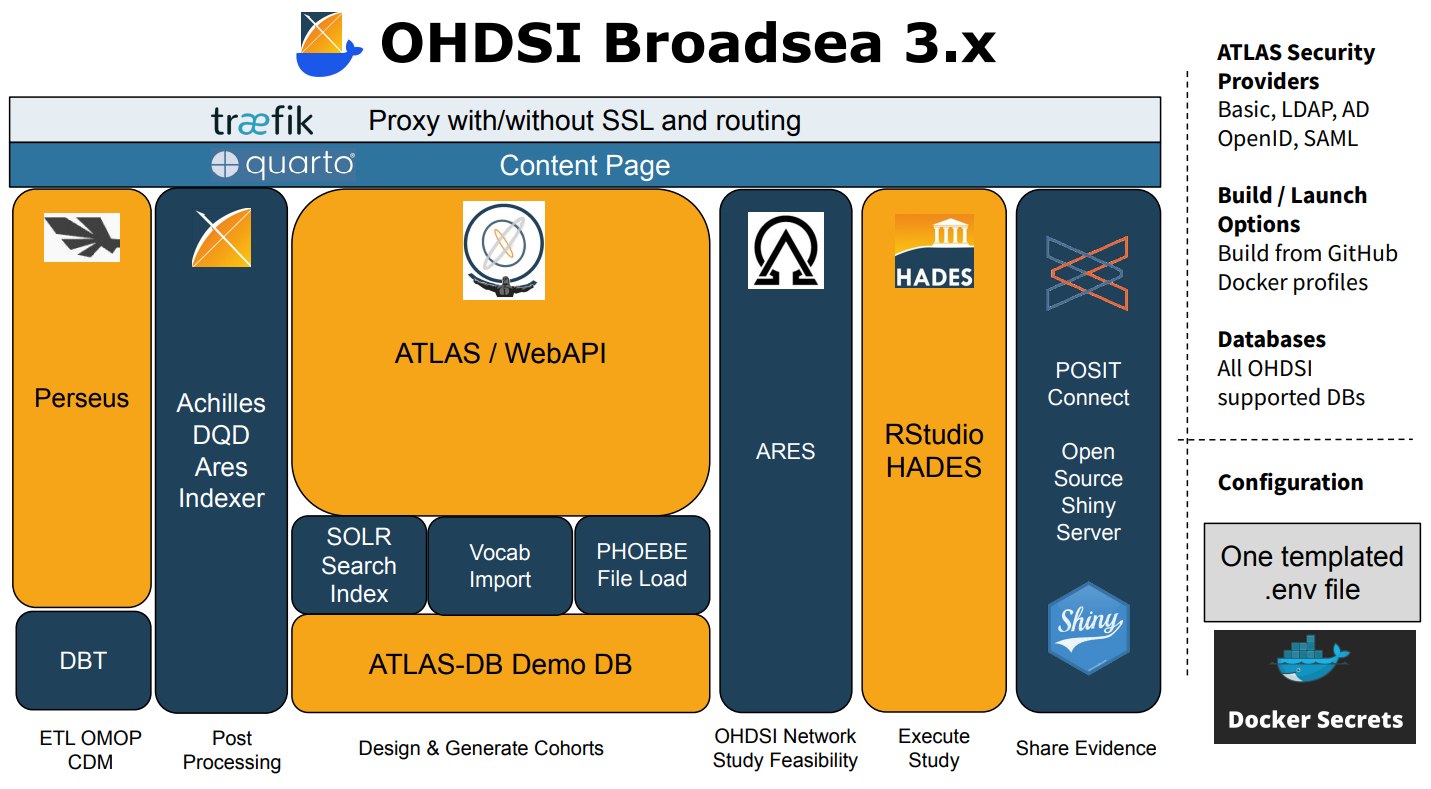
\includegraphics[width=0.90\textwidth]{figures/OHDSIBroadsea3.0.png}
    \caption{Vista general de todos los componentes de Broadsea \cite{Broadsea3PPTX}}
    \label{fig:enter-label}
\end{figure}

Este manual tan solo se centra en la instalación, despliegue y configuración de ATLAS (y la webAPI) pero las posibilidades de utilización de otras herramientas son múltiples. A partir de este momento se le denomina ATLAS Broadsea a la herramienta ATLAS que ofrece el entorno Broadsea.

\section{Docker}

Descripción del contenedor

- Funcionamiento del contenedor en github Broadsea (unica vez que se va a referenciar el link, a partir de ahi citar):

- Contenedores por defecto: ATLAS, ARES, HADES

- Perfiles:
        - por defecto
        - otros

- Archivos de configuración del entorno: docker compose, .env file

\section{BD Eunomia}

- ATLAS viene con una bd por defecto que es Eunomia
- Descripcion de eunomia (incluso del mismo data source). Numero de datos, etc.
- Vocabulario por defecto.


